\graphicspath{
  {./images/bmps/}{./images/vects/}{./images/}
  {./images/presentation/bmps/}{./images/presentation/vects/}{./images/presentation/}
  {./images/chapter00/bmps/}{./images/chapter00/vects/}{./images/chapter00/}
  {./images/chapter05/bmps/}{./images/chapter05/vects/}{./images/chapter05/}
}

\subsection{Particle Filter based Object Tracking}

\begin{frame}{Introduction}
  \begin{itemize}
   \item Inspired on \cite{danescu2012particle,broggi2013}
   \item Voxelized occupancy grid.
   \item A set of particles is assigned to each voxel.
   \item Particles are evolved, re-weighted and resampled.
   \item Object reconstruction is done by using a flood fill approach.
  \end{itemize}

  \note {
  \begin{itemize}
    \item Voxelized occupancy grid in which the world surrounding the vehicle is divided into a discrete number of voxels of the same size
    \item For each voxel, an occupancy probability is assigned, based on the number of points inside it and its neighborhood. 
    \item A set of particles will be assigned dynamically to each voxel during the execution, with a double function:
    \begin{enumerate}
	\item Denoting hypotheses (as happens with classical particle filters).
	\item Being used as the building blocks of the world model.
    \end{enumerate}
    \item At each frame, the set of particles in the previous frame is evolved using their movement model and assigned to the corresponding voxel, attending to the time passed between frames and the ego-motion. 
    \item Then, particles are re-weighted and resampled.
    \item Surviving particles are used to construct the objects that model the environment, by joining all these voxels that share a similar orientation and speed. 
    \item This object reconstruction is done by using a flood fill approach, following a similar process to that described in \cite{broggi2013}, but using the vectors of each voxel.
  \end{itemize}

  }
\end{frame}

\begin{frame}{Advantages}
  \begin{itemize}
    \item We do not need to estimate the probability distribution of the speed or the orientation.
    \item Easy encoding of the past and present knowledge from sensor data.
    \item Hierarchical object pose, orientation and speed detection.
    \item Fully 3D perception of the object detected.
    \item Simplification of the world.
    \item No color information is used.
    \item Collaborative update of the grid.
  \end{itemize}

  \note {
  \begin{itemize}
    \item \emph{We do not need to estimate the probability distribution of the speed or the orientation.} This distribution is obtained directly from the surviving particles of each voxel. 
    \item \emph{Easy encoding of the past and present knowledge from sensor data.} The usage of a voxel grid makes this easier, and allows updating it dynamically when new information is available with little computational cost.
    \item \emph{Hierarchical object pose, orientation and speed detection.} Object units are detected at lower level as individual voxels, for which we know their individual speed and pose. Joining all these voxels together, we obtain the whole obstacle, whose pose and speed is directly dependent on the voxels which compose it. 
    \item \emph{Fully 3D perception of the object detected.} No previous assumption on the shape of the obstacles is taken, providing an accurate estimation of complex obstacles. The usage of voxels instead of cuboids allows having a more clear idea of the actual shape of an obstacle, avoiding an overestimation, which is not acceptable for some applications. By using the whole dimensions, we can have an accurate idea of the 3D boundaries of an obstacle.
    \item \emph{Simplification of the world.} through the use of voxels. we can save a lot of time by using its voxel-based simplification. In the other hand, there is still information loss, but we can determine the quantity of information we are willing to loose by tuning the voxels resolution.
    \item \emph{No color information is used.} As we do not use color information coming from the input 3D point cloud, our implementation is ready to accept data from other sensors different from a stereo pair (for example, a LIDAR device) without modifications.
    \item \emph{Collaborative update of the grid.} The usage of a voxel grid also allows combining several input sources at the same time. Due to some decisions taken during the implementation of the method, it is ready for such collaborative update.
  \end{itemize}

  }
\end{frame}

\begin{frame}[plain]{Pipeline}
  \begin{center}
    \includegraphics[height=1.1\textheight]{pipeline_general_cp05}
  \end{center}
  \note{
  \begin{enumerate}
    \item \emph{3D point cloud generation.} Our implementation is able to work from data coming from any kind of sensor. Anyway, in our tests we have used point clouds obtained from stereo cameras. In this step we obtain the 3D point set that will be the input for our algorithm. At implementation level, this step is done in a separate process, so the point cloud can be used for other tasks in the system, or even be computed in a different computer or device in the future.
    \item \emph{Ego-motion.} As the car is moving, the orientation and speeds computed for the different objects is biased by the speed of the own vehicle.
    \item \emph{Voxelization.} Each of the 3D points obtained in the first step is assigned to a certain voxel. Each voxel has a certain resolution, which covers a parameterized section of the world. In our tests, we have used voxels of a resolution of $(0.25\times0.25\times0.25\,m)$ in the $X$, $Y$ and $Z$ dimensions, respectively, covering a volume going from $-4$\,m to $+4$\,m in the $X$ axis; $0$ to $+24$\,m in the $Y$ axis; and $0$ to $3.5$\,m in the $Z$ axis.
    \item \emph{Voxel pose and speed computation.} Based on a PF and in the probabilities assigned in the previous step, we calculate the pose and speed of each of the voxels in the grid.
    \item \emph{Object reconstruction.} Once we know the pose and speed of each voxel, and based on a flood fill procedure, together with the vectors already obtained, similar voxels are assigned to a common final obstacle. For each segmented object, orientation and speed is computed based on the vectors belonging to each of the associated voxels.
  \end{enumerate}
  }
\end{frame}

% \begin{frame}{3D point cloud generation}
%   \begin{center}
%     \includegraphics[width=\textwidth]{intervals}
%   \end{center}
%   \note{
%   \begin{itemize}
%    \item Comparison between ELAS, BT-SGM and Census-SGM Conf 2
%    \item Voxelization
%    \item Point cloud filtering
%   \end{itemize}
%   }
% \end{frame}
% 
% \begin{frame}{Ego-motion}
%   \begin{center}
%     \includegraphics[width=\textwidth]{tfs}
%   \end{center}
%   \note{
%   \begin{itemize}
%    \item We compared \cite{geiger2011stereoscan} with \cite{Perea2013mcl}
%   \end{itemize}
%   }
% \end{frame}

\begin{frame}[t]{Voxelization}
  \begin{overlayarea}{\textwidth}{\textheight}
  \begin{itemize}
   \item Each point $p_i = (p_x, p_y, p_z), i=1..N_p$ is assigned to the corresponding voxel $g_j=(g_w, g_l, g_h), j=1..N_g$.
   \item On each voxel, we store:
   \begin{itemize}
    \item The 3D associated points.
    \item The centroids $c=(c_x, c_y, c_z)$ of each voxel.
    \item Uncertainty of the stereo reconstruction values $\sigma_{c_x}$, $\sigma_{c_y}$ and $\sigma_{c_z}$.
    \item Weights $\omega_{occupied}$ and $\omega_{free}$.
    \item Density of 3D points $N_p$.
    \item Main orientation and speed vectors $v=(v_x, v_y, v_z)$.
    \item Stored particles $q_i = (x, y, z, v_x, v_y, v_z) \in \mathcal{Q}$.
    \item Obstacle identifier $o_i \in \mathcal{O}$.
   \end{itemize}

  \end{itemize}
%   \only<1> {
%     \vskip-4.5cm
%     \begin{block}{}
%       \begin{equation}
% 	\nonumber
% 	\begin{cases}
% 	g_w = (p_x - I_{min}(X)) / DX\\
% 	g_l = (p_y - I_{min}(Y)) / DY\\
% 	g_h = (p_z - I_{min}(Z)) / DZ
% 	\end{cases}
%       \end{equation}
%     \end{block}
%   }
%   \only<5> {
%     \vskip-2.5cm
%     \begin{block}{}
%       \begin{equation}
% 	\nonumber
% 	\begin{cases}
% 	  \sigma_{c_x}={{{c_x} \cdot \sigma_l} ~/~ {c_y}} \\
% 	  \sigma_{c_y}={{{c_y}^2 \cdot \sigma_d} ~/~ {b \cdot f}} \\
% 	  \sigma_{c_z}={{{c_z} \cdot \sigma_l} ~/~ {c_y}}
% 	\end{cases}
%       \end{equation}
%     \end{block}
%   }
%   \only<6> {
%     \vskip-2.0cm
%     \begin{block}{}
%      \tiny
%       \begin{equation}
% 	\nonumber
% 	\omega_{occupied} = p(m(w,l,h)~|~occupied) = {
% 	{\sum \limits_{w'=w-\sigma_w}^{w+\sigma_w} \sum \limits_{l'=l-\sigma_l}^{l+\sigma_l} \sum \limits_{h'=h-\sigma_h}^{h+\sigma_h} O(w',l',h')} 
% 	\over 
% 	{(2 \cdot \sigma_w + 1) \cdot (2 \cdot \sigma_l + 1) \cdot (2 \cdot \sigma_h + 1)}}
%       \end{equation}
%       \\~\\
%       \begin{equation}
% 	\nonumber \tiny
% 	\omega_{free} = p(m(w,l,h)~|~occupied) = 1 - p(m(w,l,h)~|~free)
%       \end{equation}
%     \end{block}
%   }
  \end{overlayarea}
  \note{
  }
\end{frame}

\begin{frame}{Voxelization}
  \begin{center}
    \includegraphics[height=0.7\textheight]{voxelization}
  \end{center}
\end{frame}

\begin{frame}[plain]{Voxel pose and speed computation}
  \framesubtitle{Pipeline}
  \begin{center}
    \includegraphics[height=1.1\textheight]{voxelPoseAndSpeedComputation}
  \end{center}
\end{frame}

\begin{frame}{Voxel pose and speed computation}
  \framesubtitle{Prediction}
  \begin{itemize}
   \item Particle distribution is computed considering:
   \begin{itemize}
    \item Particles motion model.
    \item Time between frames.
   \end{itemize}
   \item Ego-motion is not compensated here.
   \item The new position of each particle is $q_{t + 1} = S \cdot q_{t} + \Delta$
   
  \end{itemize}
  
  \begin{block}{}
    \footnotesize
    \begin{equation}
      \nonumber
      S =
      \left( \begin{array}{cc}
      I_{3\times3} & \Delta t \cdot I_{3\times3} \\
      0_{3x3} & I_{3\times3} \end{array} \right)
    \end{equation}
    \\~\\
    \begin{equation}
      \nonumber
      \Delta =
      \left( \begin{array}{cccccc}
      \delta x & \delta y & \delta z & \delta v_x & \delta v_y & \delta v_z
      \end{array} \right)^T
    \end{equation}
  \end{block}
  \note {
    \begin{itemize}
     \item $S$ is a state transition matrix
     \item $\delta x$, $\delta y$, $\delta z$, $\delta v_x$, $\delta v_y$ and $\delta z$, are randomly drawn from a Gaussian distribution of zero mean and a covariance matrix Q equivalent to the state transition covariance matrix of a Kalman filter.
    \end{itemize}
  }
\end{frame}

\begin{frame}[plain]{Voxel pose and speed computation}
  \framesubtitle{Weighting and resampling}
  \begin{algorithm}[H]
  \tiny
  \begin{algorithmic}
    \Function{MeasurementBasedUpdate}{$\mathcal{G}$} 
    \For {\textbf{each} voxel $g \in \mathcal{G}$}

      \Comment \textbf{Main vectors computation}
	\State \indent {$g$.computeMainVectors()}

	\Comment \textbf{Weighting}
	\State \indent Compute $N_{og}$ and $P_{og}$

	\Comment \textbf{Resampling}
	\State \indent Compute resampled number of particles $N_{rg}$
	\State \indent $N_{rg} \gets P_{og} \cdot N_g$
	\State \indent $f_g \gets {{N_{rg}} \over {N_{og}}}$
      \For {\textbf{each} particle $p$ belonging to $g$}
	\If { $f_g > 1$ } \Comment { The number of particles will be increased.}
	  \State {$F_n \gets \lfloor f_g\rfloor$} \Comment {Integer part}
	  \State {$F_f \gets f_g - \lfloor f_g\rfloor$} \Comment {Fractional part}
	  \For {$k = 1$ to $F_n - 1$}
	    \State {$g$.makeCopy($p$)}
	  \EndFor
	  \State $r \gets \text{random value in the range [0 \ldots 1]}$
	  \If {$r < F_f$}
	    \State {$g$.makeCopy($p$)}
	  \EndIf
	\Else \Comment {$f_g < 1$, the number of particles will be decreased.}
	  \State $r \gets \text{random value in the range [0 \ldots 1]}$
	  \If {$r > F_g$}
	    \State {$g$.remove($p$)}
	  \EndIf
	\EndIf
      \EndFor
    \EndFor
  \EndFunction
  \end{algorithmic}
  \end{algorithm}
  
  \begin{overlayarea}{\textwidth}{\textheight}
  \only<2> {
    \vskip-7.5cm
    \begin{block}{Main vectors computation}
      \begin{columns}
      \column{0.3\textwidth}
	\begin{center}
	  \includegraphics[width=\textwidth]{sphericalHist}\\~\\
	\end{center}
      \column{0.6\textwidth}
	\begin{itemize}
	  \item Yaw $\psi$ ($[0\dots2\pi]$) is divided in intervals of size $\Delta\psi$.
	  \begin{itemize}
	    \item Same is done for the pitch $\theta$
	  \end{itemize}
	  \item For each particle, we obtain the corresponding $\psi$ and $\theta$.	  
	\end{itemize}
      \end{columns}
    \end{block}
  }
  \only<3> {
    \vskip-7.0cm
    \begin{block}{Weighting}
      \begin{equation}\label{eq:cp05_total_posterior_probabilities}
	\nonumber \tiny
	\begin{array}{l}
	P_{og}={{\omega_{occupied} \cdot N_{og}} \over {\omega_{occupied} \cdot N_{og} + \omega_{free} \cdot N_{fg}}} \\~\\
	N_{og} = | \{ p_i \in \mathcal{P} ~|~ p_i \text{ belongs to voxel } g \} |
	\end{array}
      \end{equation}
    \end{block}
  }
  \only<4> {
  }
  \end{overlayarea}
  \note {
  \begin{itemize}
   \item In our tests, both $\Delta\psi$ and $\Delta\theta$ are set to $5^{\circ}$.
   \item For each particle, we obtain the corresponding value of $\psi$ and $\theta$, and the corresponding bin is increased in one unit.
   \item Speed and orientation will be given by the bin with the biggest number of related particles.
   \item Resampling:
   \item Unlike the method proposed by \cite{danescu2012particle}, due to optimization purposes we do not split the whole process into two different loops. Instead of having the set of particles separated from the voxels, each voxel knows exactly where its particles are. In the original algorithm, it is necessary to compute and store the value of $f_g$ for absolutely all the voxels in $\mathcal{G}$. After that, the program iterates over all the particles in $\mathcal{P}$. For each of these particles $p$, we need to know the related voxel and look for the computed value $f_g$. In our approach, we assign each particle to its voxel directly at the \emph{initialization} and \emph{prediction} steps, so we can perform all the weighting and resampling at once, saving computational time.
  \end{itemize}

  }
\end{frame}

\begin{frame}{Voxel pose and speed computation}
  \framesubtitle{Weighting and resampling}
  \begin{center}
    \includegraphics[height=0.7\textheight]{weightAndResample}
  \end{center}

\end{frame}

\begin{frame}{Voxel pose and speed computation}
  \framesubtitle{Initialization}
  \begin{itemize}
    \item Empty voxels are initialized with a number of random particles.
    \begin{itemize}
      \item First iteration.
      \item No surviving particles.
      \item A new object in the scene.
    \end{itemize}
  \end{itemize}

  \note {
    In this stage, empty voxels are initialized with a number of random particles proportional to the occupancy probability. This situation can happen due to three different reasons:
    \begin{itemize}
    \item It is the first iteration, so none of the voxels has been initialized already.
    \item After the weighting and resampling process, none of the particles survived.
    \item A new object appears in the scene, so the associated voxels were not initialized in previous iterations.
    \end{itemize}
  }
\end{frame}

\begin{frame}{Object reconstruction}
  \begin{algorithm}[H]
  \tiny
  \begin{algorithmic}[1]
  \Function{Clustering}{$\mathcal{G}$} 
  \State {$\mathcal{G'} \gets \mathcal{G}$} \Comment {$\mathcal{G'}$ is the set of not-checked voxels. }
  \For {\textbf{each} voxel $g \in \mathcal{G'}$}
    \State {$\mathcal{G'} \gets \mathcal{G'} - g$}
    \State {$o \gets \text{ new object containing }g$}
    \State {$\text{insert } g \text{ in } queue$}
    \While {$queue \ne \emptyset$}
      \State {$g' \gets \text{extract first element from the } queue$}
      \For {\textbf{each} $\{ g'' | g'' \in o\} \in N(g')$}
	\If {$ f_1(o,g) < \tau_{v} \textbf{ and } f_2(o,g) < \tau_{\psi} \textbf{ and } f_3(o,g) < \tau_{\theta} $}
	  \State {$\text{insert } g'' \text{ in } o$}
	  \State {$\text{insert } g'' \text{ in } queue$}
	\EndIf
      \EndFor
    \EndWhile
    \If {$|o| >= \tau_{min\_voxels\_per\_obstacle} \textbf{ and } o.sz(Z) >= \tau_{min\_obstacle\_height} \textbf{ and } o.min(Z) == I_{min}(Z) $}
	\State {$o \text{.updateVectors()}$}
	\State {$\text{insert } o \text{ in } \mathcal{O}$}
    \EndIf
  \EndFor
  \EndFunction
  \end{algorithmic}
  \end{algorithm}

  \begin{overlayarea}{\textwidth}{\textheight}
    \only<2> {
    \vskip-4.0cm
    \begin{block}{Similarity function}
      \begin{equation}
	\nonumber
	\begin{array}{l}
	  f_1(o,g)=\| |\vec{v}|_o - |\vec{v}|_g \|\\
	  f_2(o,g)=\| \psi_o - \psi_g \|\\
	  f_3(o,g)=\| \theta_o - \theta_g \|
	\end{array}
      \end{equation}
    \end{block}
    }
    \only<3> {
    }
  \end{overlayarea}

  \note {
    Once an obstacle is about to be added to the final set of obstacles, this list will be used for updating the information related to the obstacle centroid, speed and limits on each dimension
    
    An obstacle is accepted in the final list if:

    \begin{itemize}
    \item It is big enough. That is, if the number of voxels (which is directly proportional to its volume) is over the user-defined parameter $\tau_{min\_voxels\_per\_obstacle}$.
    \item It is tall enough. The minimal height is controlled by the parameter\\ $\tau_{min\_obstacle\_height}$
    \item The obstacle is on the ground. This helps to remove flying obstacles like traffic lights or the top of some trees, in which we are not interested.
    \end{itemize}
  }
\end{frame}

\begin{frame}{Obstacle vectors computation}
  
  \begin{block}{}
    \begin{equation}
      \nonumber \tiny
      \begin{cases}
	o_{vx} = {{\sum\limits_{g \in \mathcal{G}_o} g_{vx}} \over {|\mathcal{G}_o|}} - ego_{vx}\\
	o_{vy} = {{\sum\limits_{g \in \mathcal{G}_o} g_{vy}} \over {|\mathcal{G}_o|}} - ego_{vy}\\
	o_{vz} = {{\sum\limits_{g \in \mathcal{G}_o} g_{vz}} \over {|\mathcal{G}_o|}} - ego_{vz}
      \end{cases}
    \end{equation}
  \end{block}
  
  \begin{figure}
    \includegraphics[height=0.5\textheight]{fakePointCloud}
  \end{figure}


  \note {
  
  }
\end{frame}

\begin{frame}{Particle Filter based Object Tracking}
  \begin{center}
    \includemovie[autoplay, repeat, controls]{\textwidth}{0.8\textheight}{/home/nestor/Seafile/Videos/Tesis/cp05/PfAndVoxelPipeline.mp4}
  \end{center}
\end{frame}

\begin{frame}{Obstacle detection and tracking}
  \begin{itemize}
  \item Goals:
    \begin{enumerate}
      \item Good obstacle detection rate. \only<2->{\textcolor{green}{\cmark}}
      \item Obstacle localization. \only<3->{\textcolor{green}{\cmark}}
      \item Real time. \only<4->{\textcolor{green}{\cmark}}
      \item Environment conditions independence. \only<5->{\textcolor{green}{\cmark}}
      \item Tracking capabilities. \only<6->{\textcolor{green}{\cmark}}
      \item Moving cameras. \only<7->{\textcolor{green}{\cmark}}
    \end{enumerate}
  \end{itemize}
\end{frame}